\documentclass[12pt]{article}
\usepackage{fontspec}
\usepackage{xcolor}
\usepackage{listings}
\usepackage[justification=centering]{caption}
\usepackage{subcaption}
\usepackage{cite}
\usepackage{amssymb}
\usepackage{amsmath}
\usepackage{amsthm}
\usepackage{mathtools}
\usepackage{bussproofs}
\usepackage{tikz}
\usepackage{float}
\usepackage{graphicx}
\usepackage{algorithm}
\usepackage[noend]{algpseudocode}
\usepackage{array}
\usepackage{stmaryrd}
\usepackage{pifont}
\usepackage{enumitem}
\usepackage{extarrows}

\usepackage{hyperref}
\usepackage[capitalise]{cleveref}
%% \usepackage{chngcntr}

\newcommand{\rulehskip}{\hskip 1.5em}
\newcommand{\rulevspace}{\vspace{1em}}

\mathchardef\mhyphen="2D

\theoremstyle{definition}

\newtheorem{definition}{Definition}
\newtheorem{theorem}{Theorem}
\newtheorem{lemma}{Lemma}
\newtheorem{prop}{Proposition}

%% \counterwithin{lemma}{section}

\newcommand{\textdef}[1]{\textit{#1}}

\newcommand{\imm}{{\textrm IMM}~}

% inline code 
\newcommand{\code}[1]{\texttt{#1}}

% tuple with angle brackets
\newcommand{\tup}[1]{\langle #1 \rangle}

% semantics brackets
\newcommand{\sem}[1]{\llbracket #1 \rrbracket}

% equality by definition
\newcommand{\defeq}{\triangleq}

% function arrow
\newcommand{\fun}{\rightarrow}

% partial function arrow
\newcommand{\pfun}{\rightharpoonup}

% some math sets
\newcommand{\N}{{\mathbb{N}}}
\newcommand{\Q}{{\mathbb{Q}}}

% domain/codomain notation
\newcommand{\dom}[1]{\textit{dom}{({#1})}}
\newcommand{\codom}[1]{\textit{codom}{({#1})}}

\newcommand{\lca}{\textit{lca}}

% some logical notation
%\newcommand{\implies}{{\Rightarrow}}
%\newcommand{\iff}{{\Leftrightarrow}}

% check-mark and cross-mark
\newcommand{\cmark}{\text{\color{green}\ding{51}}}
\newcommand{\xmark}{\text{\color{red}\ding{55}}}

% event structure
\newcommand{\lES}{S}
% event structure's execution

% execution graph
\newcommand{\lG}{G}
% covered/issued events
\newcommand{\lC}{C}
\newcommand{\lI}{I}
% mapping between events
\newcommand{\lM}{m}
\newcommand{\lMC}{m_{c}}
\newcommand{\lMI}{m_{i}}

% event set
\newcommand{\lE}{{\mathtt{E}}}
\newcommand{\lEi}[1]{\lE_{#1}}
\newcommand{\lEo}{\lEi{0}}
\newcommand{\lEs}{\widehat{{\mathtt{E}}}}
\newcommand{\lEsi}[1]{\lEs_{#1}}
\newcommand{\lEso}{\lEsi{0}}
\newcommand{\lR}{{\mathtt{R}}}
\newcommand{\lW}{{\mathtt{W}}}
\newcommand{\lF}{{\mathtt{F}}}
\newcommand{\lX}{{\mathtt{X}}}

\newcommand{\lEsqeq}[1]{{\lE^{\sqsupseteq#1}}}
\newcommand{\lRsqeq}[1]{{\lR^{\sqsupseteq#1}}}
\newcommand{\lWsqeq}[1]{{\lW^{\sqsupseteq#1}}}
\newcommand{\lFsqeq}[1]{{\lF^{\sqsupseteq#1}}}

% labeling of events
\newcommand{\Tid}{\mathsf{Tid}}
\newcommand{\Loc}{\mathsf{Loc}}
\newcommand{\Val}{\mathsf{Val}}
\newcommand{\Bool}{\mathsf{Bool}}
\newcommand{\Lab}{\mathsf{Lab}}
\newcommand{\Mod}{\mathsf{Mod}}
\newcommand{\Cont}{\kappa}
\newcommand{\Scp}{\mathsf{Scope}}
\newcommand{\Path}{\pi}
\newcommand{\Prog}{\mathsf{prog}}
\newcommand{\Execs}[1]{\Psi_{#1}}

\newcommand{\lLAB}{{\mathtt{lab}}}
\newcommand{\lTID}{{\mathtt{tid}}}
\newcommand{\lTYP}{{\mathtt{typ}}}
\newcommand{\lLOC}{{\mathtt{loc}}}
\newcommand{\lMOD}{{\mathtt{mod}}}
\newcommand{\lSCP}{{\mathtt{scp}}}
\newcommand{\lCONT}{{\mathtt{K}}}
\newcommand{\lVALR}{{\mathtt{val_r}}}
\newcommand{\lVALW}{{\mathtt{val_w}}}
\newcommand{\lINIT}{{\mathtt{init}}}
\newcommand{\lSN}{{\mathtt{sn}}}
\newcommand{\lPC}{{\mathtt{pc}}}
\newcommand{\lPREV}{{\mathtt{prev}}}

\newcommand{\lMASK}{{\mathtt{Mask}}}
\newcommand{\lVIS}{{\mathtt{Vis}}}

% simulation relation 
\newcommand{\simR}{\mathcal{I}}
\newcommand{\simRb}{\mathcal{I}_{base}}
\newcommand{\simRw}{\mathcal{I}_{weak}}

\newcommand{\nextset}{{\mathtt{Next}}}
\newcommand{\coverable}{{\mathtt{Coverable}}}
\newcommand{\issuable}{{\mathtt{Issuable}}}
\newcommand{\front}{\phi}
\newcommand{\forward}{{\mathtt{Forward}}}
\newcommand{\cert}{{\mathtt{cert}}}
\newcommand{\certify}{{\mathtt{Certify}}}

%\newcommand{\lCERTIFY}{{\mathtt{Certify}}}

\newcommand{\trstep}{\longrightarrow}
\newcommand{\esbstep}[1]{\xLongrightarrow{#1}}
\newcommand{\esstep}[1]{\xlongrightarrow{#1}}
\newcommand{\esstepstar}{\longrightarrow^*}

\newcommand{\ESle}{\preceq}
\newcommand{\ESbasicstep}[1]{\xLongrightarrow{#1}}
\newcommand{\ESstep}[1]{\xlongrightarrow{#1}}
\newcommand{\ESstepstar}{\longrightarrow^*}

\newcommand{\rlab}[3]{\lR^{#1}({#2},{#3})}
\newcommand{\wlab}[3]{\lW^{#1}({#2},{#3})}
\newcommand{\flab}[1]{\lF^{#1}}

\newcommand{\Ex}{{\mathtt{ex}}}
\newcommand{\NotEx}{{\mathtt{not \mhyphen ex}}}
\newcommand{\rlabExExpl}[4]{\lR_{#4}^{#1}({#2},{#3})}
\newcommand{\rlabEx}[3]{\rlabExExpl{#1}{#2}{#3}{\Ex}}

%% \newcommand{\rlabS}[3]{\lR^{#3}({#1},{#2})}
%% \newcommand{\wlabS}[3]{\lW^{#3}({#1},{#2})}
%% \newcommand{\flabS}[1]{\lF^{#1}}

% some predefined relations
\colorlet{colorPO}{gray!60!black}
\colorlet{colorPPO}{magenta}
\colorlet{colorRF}{green!60!black}
\colorlet{colorJF}{green!40!black}
\colorlet{colorRMW}{olive!70!black}
\colorlet{colorCF}{red!60!black}
\colorlet{colorEW}{brown}
\colorlet{colorMO}{orange!60!black}
\colorlet{colorRB}{purple}
\colorlet{colorECO}{red!80!black}
\colorlet{colorRSEQ}{cyan}
\colorlet{colorRELP}{cyan}
\colorlet{colorSW}{blue!40!black}
\colorlet{colorHB}{blue}
\colorlet{colorSCB}{violet}
\colorlet{colorPSC}{violet}
\colorlet{colorFSC}{violet}
\colorlet{colorSC}{violet}
\colorlet{colorWGR}{magenta!40!black}
\colorlet{colorDEV}{magenta}
\colorlet{colorINCL}{magenta!70!black}
\colorlet{colorOBS}{green!40!black}
\colorlet{colorCA}{teal}
\colorlet{colorDEPS}{violet!60!black}
\colorlet{colorDETOUR}{teal}
\colorlet{colorBOB}{gray!80!black}

\newcommand{\lPO}{{\color{colorPO}\mathtt{po}}}
\newcommand{\lPPO}{{\color{colorPPO}\mathtt{ppo}}}
\newcommand{\lRF}{{\color{colorRF}\mathtt{rf}}}
\newcommand{\lJF}{{\color{colorRF}\mathtt{jf}}}
\newcommand{\lRMW}{{\color{colorRMW}\mathtt{rmw}}}
\newcommand{\lCF}{{\color{colorCF}\mathtt{cf}}}
\newcommand{\lEW}{{\color{colorEW}\mathtt{ew}}}
\newcommand{\lMO}{{\color{colorMO}\mathtt{mo}}}
\newcommand{\lRB}{{\color{colorRB}\mathtt{rb}}}
\newcommand{\lECO}{{\color{colorECO}\mathtt{eco}}}

\newcommand{\lRSEQ}{{\color{colorRSEQ}\mathtt{rseq}}}
\newcommand{\lRELP}{{\color{colorRELP}\mathtt{relp}}}
\newcommand{\lSW}{{\color{colorSW}\mathtt{sw}}}
\newcommand{\lHB}{{\color{colorHB}\mathtt{hb}}}

\newcommand{\ocl}{{\textrm OpenCL}}
\newcommand{\ptx}{{\textrm PTX}}
\newcommand{\lSWocl}{{\color{colorSW}\mathtt{sw_\ocl}}}
\newcommand{\lSWptx}{{\color{colorSW}\mathtt{sw_\ptx}}}

\newcommand{\lSCB}{{\color{colorSCB} \mathtt{scb}}}
\newcommand{\lPSCB}{\lPSC_{\rm base}}
\newcommand{\lPSCF}{\lPSC_\lF}
\newcommand{\lFSC}{{\color{colorFSC}\mathtt{fsc}}}
\newcommand{\lPSC}{{\color{colorPSC}\mathtt{psc}}}
\newcommand{\lSC}{{\color{colorSC}\mathtt{sc}}}

\newcommand{\lWGR}{{\color{colorWGR}\mathtt{wgr}}}
\newcommand{\lWGRi}[1]{{\color{colorWGR}\mathtt{wgr}_{#1}}}
\newcommand{\lDEV}{{\color{colorDEV}\mathtt{dev}}}
\newcommand{\lINCL}{{\color{colorINCL}\mathtt{incl}}}
\newcommand{\lHBINCL}{\lHB_{\lINCL}}

\newcommand{\lOBS}{{\color{colorOBS}\mathtt{obs}}}
\newcommand{\lCA}{{\color{colorCA}\mathtt{ca}}}
\newcommand{\lCAB}{\lCA_{\rm base}}

\newcommand{\lCTRL}{{{\color{colorDEPS}\mathtt{ctrl}}}}
\newcommand{\lDATA}{{{\color{colorDEPS}\mathtt{data}}}}
\newcommand{\lADDR}{{{\color{colorDEPS}\mathtt{addr}}}}
\newcommand{\lCASDEP}{{{\color{colorDEPS}\mathtt{casdep}}}}
\newcommand{\lDEPS}{{\color{colorDEPS}\mathtt{dep}}}

\newcommand{\lBOB}{{\color{colorBOB}\mathtt{bob}}}
\newcommand{\lDETOUR}{{\color{colorDETOUR}\mathtt{detour}}}

\newcommand{\lmakeE}[1]{#1\mathtt{e}}
\newcommand{\lRFE}{\lmakeE{\lRF}}
\newcommand{\lCOE}{\lmakeE{\lCO}}
\newcommand{\lRBE}{\lmakeE{\lRB}}
\newcommand{\lMOE}{\lmakeE{\lMO}}

\newcommand{\lmakeI}[1]{#1\mathtt{i}}
\newcommand{\lRFI}{\lmakeI{\lRF}}
\newcommand{\lCOI}{\lmakeI{\lCO}}
\newcommand{\lFRI}{\lmakeI{\lFR}}

\newcommand{\lmakeLoc}[1]{#1_{|loc}}

%% memory orders
\newcommand{\na}{\mathtt{na}}
\newcommand{\pln}{\mathtt{pln}}
\newcommand{\rlx}{\mathtt{rlx}}
\newcommand{\rel}{{\mathtt{rel}}}
\newcommand{\acq}{{\mathtt{acq}}}
\newcommand{\con}{{\mathtt{con}}}
\newcommand{\acqrel}{{\mathtt{acqrel}}}
\newcommand{\relAcq}{\acqrel}
\newcommand{\sco}{{\mathtt{sc}}}

%% scopes
\newcommand{\wgr}{\mathtt{wgr}}
\newcommand{\dev}{\mathtt{dev}}
\newcommand{\sys}{\mathtt{sys}}

%% tikz stuff

\newcommand{\event}[3]{#1#2#3}
\tikzset{
   every path/.style={>=stealth},
   po/.style={->,color=colorPO,,shorten >=-0.5mm,shorten <=-0.5mm},
   rf/.style={->,color=colorRF,dashed,,shorten >=-0.5mm,shorten <=-0.5mm},
   rb/.style={->,color=colorRB,thick,shorten >=-0.5mm,shorten <=-0.5mm},
   mo/.style={->,color=colorMO,dotted,thick,shorten >=-0.5mm,shorten <=-0.5mm},
   sw/.style={->,color=colorSW,dashed,thick,shorten >=-0.5mm,shorten <=-0.5mm},
   obs/.style={->,color=colorOBS,dashed,,shorten >=-0.5mm,shorten <=-0.5mm},
   no/.style={->,dotted,thick,shorten >=-0.5mm,shorten <=-0.5mm},
   deps/.style={->,color=colorDEPS,dotted,thick,shorten >=-0.5mm,shorten <=-0.5mm},
   wgr/.style={fill=colorWGR, opacity=0.1}
}

%% parallel threads listings

\newcommand{\inarr}[1]{\begin{array}{@{}l@{}}#1\end{array}}
\newcommand{\inarrII}[2]{\begin{array}{@{}l@{~~}||@{~~}l@{}}\inarr{#1}&\inarr{#2}\end{array}}
\newcommand{\inarrIII}[3]{\begin{array}{@{}l@{~~}||@{~~}l@{~~}||@{~~}l@{}}\inarr{#1}&\inarr{#2}&\inarr{#3}\end{array}}
\newcommand{\inarrIV}[4]{\begin{array}{@{}l@{~~}||@{~~}l@{~~}||@{~~}l@{~~}||@{~~}l@{}}\inarr{#1}&\inarr{#2}&\inarr{#3}&\inarr{#4}\end{array}}
\newcommand{\inarrV}[5]{\begin{array}{@{}l@{~~}||@{~~}l@{~~}||@{~~}l@{~~}||@{~~}l@{~~}||@{~~}l@{}}\inarr{#1}&\inarr{#2}&\inarr{#3}&\inarr{#4}&\inarr{#5}\end{array}}

%% instructions for listings

\newcommand{\valueRead}[1]{{// #1}}

\newcommand{\fence}{\texttt{fence}}
\newcommand{\readInstS}[3]{#2 \;:=^{#1}\;[#3]}
\newcommand{\writeInstS}[3]{[#2] \;:=^{#1}\;#3}
\newcommand{\fenceInstS}[1]{\fence^{#1}}

%% axiom labels

\newcounter{mylabelcounter}

\makeatletter
\newcommand{\labelAxiom}[2]{%
\hfill{\normalfont\textsc{(#1)}}\refstepcounter{mylabelcounter}
\immediate\write\@auxout{%
  \string\newlabel{#2}{{\unexpanded{\normalfont\textsc{#1}}}{\thepage}{{\unexpanded{\normalfont\textsc{#1}}}}{mylabelcounter.\number\value{mylabelcounter}}{}}
}%
}
\makeatother

%% warning

\colorlet{colorWARNING}{yellow!90!black}

\newcommand{\warning}[1]{{\color{colorWARNING}\texttt{WARNING}}: #1}
\newcommand{\app}[1]{{\color{blue}\textbf{ANTON: #1}}}
\newcommand{\note}[1]{{\color{cyan}\textbf{EVG: #1}}}
\newcommand{\todo}[1]{{\color{red}\textbf{TODO: #1}}}


\begin{document}

\begin{center}
{\center \LARGE Compiling Event Structures to the Intermediate Memory Model }
\end{center}

\section{Executions}

\begin{definition}
  \label{def:exec}
  
  An execution graph $X$ is a tuple $\tup{\lE, \lLAB, \lRF, \lMO}$ where:
  \begin{itemize}

    \item $\lE$ is a set of events. 
    An event is either:
    \begin{itemize}
      \item an \emph{initialization} event $\tup{\lINIT~x}$ where $x \in \Loc$;
      \item a \emph{non-initialization} event $\tup{i, n}$ where $i \in \Tid$ and $n \in \Q$.
    \end{itemize}
    Given this representation one could derive the following notions:
    \begin{itemize}

      \item $\lEo \defeq \{e \in E ~|~ \exists{x} \in \Loc ~.~ e = \tup{\lINIT~x}\}$ ---
      a set of \emph{initialization events};

      \item $\lTID : \lX \fun \Tid$ ---
      a function, that assigns a \emph{thread identifier} to every event, s.t. \\
      \begin{equation*}
        \begin{split}
          \forall{e} ~.~
          & (\exists{x \in \Loc} ~.~ e = \tup{\lINIT~x} \Rightarrow \lTID(e) = 0) \wedge \\ \wedge
          & (\exists{i \in \Tid, n \in \N} ~.~ e = \tup{i, n} \Rightarrow \lTID(e) = i)
        \end{split}
      \end{equation*}
      
      \item $\lPO \subseteq \lE \times \lE$ a \emph{program order} relation s.t. \\
      \begin{equation*}
        \begin{split}
          & \tup{e_1, e_2} \in \lPO \Leftrightarrow \\
          & \Leftrightarrow (e_1 \in \lEo \wedge e_2 \not\in \lEo) \vee 
          (e_1, e_2 \not\in \lEo \wedge \lTID(e_1) = \lTID(e_2) \wedge
          \lSN(e_1) < \lSN(e_2))
        \end{split}
      \end{equation*}
      where $\lSN(\tup{i, n}) = n$.

      Note that $\lPO$ totally orders all events within a thread.
    \end{itemize}

    \item $\lLAB \defeq \lE \fun \Lab$ --- function that assigns a label to every event.
    Labels are of one of the following forms:
    \begin{itemize}
      \item $\rlabExExpl{o}{x}{v}{\mathtt{f}}$ --- a read, where
        $x \in \Loc$, $v \in \Val$, $o \in \Mod$ 
        and $\mathtt{f} \in \{\Ex, \NotEx\}$ is an exclusive flag 
        (we will denote exclusive reads as $\rlabEx{o}{x}{v}$,
        for non-exclusive reads we will omit the flag);
      \item $\wlab{o}{x}{v}$ --- a write, where $x \in \Loc$, $v \in \Val$, $o \in \Mod$;
      \item $\flab{o}$ --- a fence, where $o \in Mod$.
    \end{itemize}
    We assume that $\forall{e} \in \lEo. \; \lLAB(e) = \wlab{\rlx}{x}{0}$.
    $\lLAB$ induces the following functions:
    \begin{itemize}
      \item $\lTYP \defeq \lE \fun \{\lR, \lW, \lF\}$ --- assigns a type to every event;
      \item $\lLOC \defeq \lE \pfun \Loc $ --- returns the location of event (when applicable);
      \item $\lVALR \defeq \lE \pfun \Val$ --- returns the read value of event (when applicable);
      \item $\lVALW \defeq \lE \pfun \Val$ --- returns the written value of event
        (when applicable);
      \item $\lMOD = G.\lE \rightarrow \Mod$ --- returns the associated memory order parameter.
        Additionally, $\lMOD$ satisfies the following constraints:
        \begin{itemize}
        \item $e \in \lR \Rightarrow \lMOD(e) \in \{ \rlx, \acq, \sco \}$;
        \item $e \in \lW \Rightarrow \lMOD(e) \in \{ \rlx, \rel, \sco \}$;
        \item $e \in \lF \Rightarrow \lMOD(e) \in \{ \rlx, \acqrel, \sco \}$.
        \end{itemize}
    \end{itemize}

    Pairs of events, consisting of an exclusive read followed by exclusive write in $\lPO_{imm}$,
    that operate on the same location,
    form a \emph{read-modify-write} relation:
    \begin{itemize}
      \item $\lRMW \defeq [\lR_{\Ex}];(\lPO_{imm} \cap =_{\lLOC});[\lW_{\Ex}]$.
    \end{itemize}

    \item $\lRF \subseteq [\lW];=_{\lLOC};[\lR]$ --- \emph{reads-from} relation,
    which the following hold for:
    \begin{itemize}
      \item $\forall{\tup{a, b}} \in \lRF. \; \lVALW(a) = \lVALR(b)$;
      \item $\forall{a_1, a_2, b}. \;
        \tup{a_1, b} \in \lRF \wedge \tup{a_2, b} \in \lRF \Rightarrow a_1 = a_2.$
    \end{itemize}
    
    \item $\lMO \subseteq \lW \times \lW$ --- \emph{modification order},
    which is a strict partial order among write operations.

  \end{itemize}

  Using the definition of relations given above,
  we will also derive the following relations:
  \begin{itemize}
    \item $\lRB \defeq (\lRF^{-1};\lMO)$ --- \emph{reads before};
    \item $\lECO \defeq (\lRF \cup \lRB \cup \lMO)^+$ --- \emph{extended coherence order}.
  \end{itemize}

\end{definition}


\begin{definition}
  Giving an execution $X$ we define the \emph{happens-before} relation $\lHB$
  using auxililarly relations: 
  $\lRSEQ$ --- release sequence,
  $\lRELP$ --- release prefix and
  $\lSW$ --- synchronize-with.
  \begin{itemize}
  \item $\lRSEQ \defeq [\lWsqeq{rlx}];(\lmakeLoc{\lPO};[\lWsqeq{rlx}] \cup 
    (\lmakeLoc{\lPO^?};[\lWsqeq{\rlx}];\lRF;\lRMW)^*)$;
  \item $\lRELP \defeq [\lEsqeq{rel}];([\lW] \cup [\lF];\lPO);\lRSEQ$;
  \item $\lSW \defeq \lRELP; (\lRFI \cup \lmakeLoc{\lPO^?};\lRFE); ([\lR] \cup \lPO;[\lF]);[\lEsqeq{\acq}]$;
  \item $\lHB \defeq (\lPO \cup \lSW)^+$.
  \end{itemize}
\end{definition}

\begin{definition}
  We will call an execution graph $X$ \emph{consistent} if the following properties hold:
  \begin{itemize}
    \item $X.\lMO^= = [X.\lW];=_{\lLOC};[X.\lW]$
    \item $X.\lRMW \cap (X.\lRB;X.\lMO) = \emptyset$
    \item $X.\lHB;X.\lECO^?$ is irreflexive.
  \end{itemize}
\end{definition}

\begin{definition}
  A function $O : \Loc \fun \Val$ is an \emph{outcome} 
  of a consistent execution graph $X$
  if for every $x \in \Loc$ either $O(x) = X.\lVALW(w)$ 
  for some $X.\lMO$-maximal write event $w$, 
  or $O(x) = 0$ and $X.\lW_x = \emptyset$.
\end{definition}

\section{Intermediate Memory Model}

\begin{definition}
  An \imm execution graph $G$ is a tuple \\
  $\tup{X, \lDATA, \lADDR, \lCTRL, \lCASDEP}$ where:
  \begin{itemize}
    \item $X$ is a regular execution graph (from the definition \ref{def:exec}).
      We will omit the $X$ when refering to its components in the context of $G$
      (e.g. we will write $G.\lPO$ instead of $G.X.\lPO$).
    \item $\lDATA \subseteq \lR \times \lW$ --- data dependency.
    \item $\lADDR \subseteq \lR \times (\lR \cup \lW)$ --- address dependency.
    \item $\lCTRL \supseteq \lCTRL; \lPO$ --- control dependency.
    \item $\lCASDEP \subseteq [R];\lPO;[R^{\Ex}]$ --- CAS dependency.
  \end{itemize}

  We will also need several derived relations:
  \begin{itemize}
    \item $\lBOB \defeq
      \lPO;[\lW^{\rel}] \cup [R^{\acq}];\lPO \cup \lPO;[\lF] \cup [\lF];\lPO \cup [\lW^{\rel}];\lPO_{\lLOC};[\lW]$;
    \item $\lDEPS \defeq \lDATA \cup \lCTRL \cup \lADDR;\lPO^? \cup \lCASDEP \cup [\lR_{\Ex}];\lPO$;
    \item $\lPPO \defeq [\lR];(\lDEPS \cup \lRFI)^+;[\lW]$;
    \item $\lDETOUR \defeq (\lMOE;\lRFE) \cap \lPO$.
  \end{itemize}

\end{definition}

\begin{definition}
  An \imm execution graph $G$ is called \emph{\imm-consistent} if the following properties hold:
  \begin{itemize}
    \item $G.X$ is a consistent execution;
    \item $G.\lRFE \cup G.\lBOB \cup G.\lPPO \cup G.\lDETOUR$ is acyclic.
  \end{itemize}
\end{definition}

\section{Event Structure Model}

\begin{definition}
  \label{def:es}
  
  An \emph{event structure} $S$ is a tuple
  $\tup{\lEs, \lJF, \lEW, \lMO}$ where:
  \begin{itemize}
    \item $\lEs$ is a set of \emph{s-events}.
    An s-event $\hat{e} \in \lEs$ is a tuple $\tup{i, \Path}$
    where $i \in \Tid$ and $\Path = (l_1, \dots, l_n)$ is a finite non-empty sequence of labels.
    We will also distinguish a set of initialization s-events $\lEo$.
    For these events thread identifier is equal to 0 and
    sequence of labels consists of single label, which is a relaxed write:
    \begin{equation*}
      \forall{\hat{e} \in \lEo} ~.~ \exists{x \in \Loc} ~.~ \hat{e} = \tup{0, \wlab{\rlx}{x}{0}}
    \end{equation*}
    Giving $\lEs$ we will also derive the following definitions:

    \begin{itemize}
      
      \item $\lTID : \lE \fun \Tid$ --- function that assigns a thread id to every s-event.
      \begin{equation*}
        \lTID(\tup{i, \Path}) \defeq i
      \end{equation*}
      Given thread id $i \in \Tid$ we will denote by $\lEi{i}$ the set of all events belonging 
      to $i^{th}$ thread, that is $\lEi{i} \defeq \{e \in \lE ~|~ \lTID(e) = i\}$.
      We will also distinguish a set of initialization events $\lEo$.
      For these events thread identifier is equal to 0 and
      sequence of labels consists of single label, which is a relaxed write:
      \begin{equation*}
        \forall{\hat{e} \in \lEo} ~.~ \exists{x \in \Loc} ~.~ \hat{e} = \tup{0, \wlab{\rlx}{x}{0}}
      \end{equation*}

      \item $\lLAB \defeq \lE \fun \Lab$ --- function that assigns a label to every s-event,
      defined as follow:
      \begin{equation*}
        \lLAB(\tup{i, (l_1, \dots, l_n)}) \defeq l_n
      \end{equation*}
      This function iduces $\lTYP$, $\lLOC$, $\lVALR$, $\lVALW$ and $\lMOD$
      as in the definition \ref{def:exec} of execution graph.

      \item Program order defined as follows:
      \begin{equation*}
        \begin{split}
        & \tup{\hat{e_1}, \hat{e_2}} \in \lPO \Leftrightarrow \\
        &   \Leftrightarrow (\hat{e_1} \in \lEso \wedge \hat{e_2} \not\in \lEso) \vee (\Path(\hat{e_1}) \prec \Path(\hat{e_2}))
        \end{split}
      \end{equation*}
      where $\prec$ is a lexicographical order.

      \item $\lCF \subseteq [\lE];=_{\lTID};[\lE]$ --- \emph{conflict relation},
      which binds two events whenever they are issued from the same thread but
      in different execution branches.
      More formally:
      \begin{equation*}
        % \tup{\hat{e_1}, \hat{e_2}} \in \lCF \Leftrightarrow
      \end{equation*}

      \item $\lRMW \subseteq [\lR_{\Ex}];(\lPO_{imm} \cap =_{\lLOC});[\lW_{\Ex}]$ ---
      \emph{read-modify-write pairs}.

    \end{itemize}
     

    \item $\lJF \subseteq [\lW];=_{\lLOC};[\lR]$ --- \emph{justified-from} relation,
    which the following
    hold for:
    \begin{itemize}
    \item $\forall{\tup{a, b}} \in \lJF. \; \lVALW(a) = \lVALR(b)$;
    \item $\forall{a_1, a_2, b}. \;
      \tup{a_1, b} \in \lJF \wedge \tup{a_2, b} \in \lJF \Rightarrow a_1 = a_2.$
    \end{itemize}
    
  \item $\lEW \subseteq \lW \times \lW$ --- is the \emph{equal write} relation, 
    which is an irreflexive, symmetric and transitive relation between conflicting writes on the
    same location writing same values 
    (that is $\lEW(e_1, e_2) \Rightarrow \lVALW(e_1) = \lVALW(e_2)$).
    Given $\lJF$, $\lEW$ and $\lCF$ we will also define a derived \emph{read from} relation:
    \begin{itemize}
      \item $\lRF \defeq \lEW^?;\lJF \setminus \lCF$
    \end{itemize}
  \item $\lMO \subseteq \lW \times \lW$ --- \emph{modification order},
    which is a strict partial order.
  \end{itemize}
\end{definition}

\begin{definition}
  Using the primitive relations of an event structure $\lES$,
  we define following derived relations:
  \begin{itemize}
    \item $\lES.\lRB \defeq (\lES.\lRF^{-1};\lES.\lMO) \setminus \lES.\lCF^?$ --- 
      \emph{reads before};
    \item $\lES.\lECO \defeq (\lES.\lRF \cup \lES.\lRB \cup \lES.\lMO)^+$ --- 
      \emph{extended coherence order}.
  \end{itemize}
\end{definition}

\begin{definition}
  Giving an event structure $\lES$ we define the \emph{happens-before} relation $\lHB$
  using auxililarly relations: 
  $\lRSEQ$ --- release sequence,
  $\lRELP$ --- release prefix and
  $\lSW$ --- synchronize-with.
  \begin{itemize}
  \item $\lRSEQ \defeq [\lWsqeq{rlx}];(\lmakeLoc{\lPO};[\lWsqeq{rlx}] \cup 
    (\lmakeLoc{\lPO^?};[\lWsqeq{\rlx}];\lJF;\lRMW)^*)$;
  \item $\lRELP \defeq [\lEsqeq{rel}];([\lW] \cup [\lF];\lPO);\lRSEQ$;
  \item $\lSW \defeq \lRELP; (\lRFI \cup \lmakeLoc{\lPO^?};\lRFE); [\lR \cup \lPO;[\lF]);[\lEsqeq{\acq}]$;
  \item $\lHB \defeq (\lPO \cup \lSW)^+$.
  \end{itemize}
\end{definition}


\begin{definition}
  For an event structure $S$ the set of its visible events $\lVIS(S)$ defined as follow:
  \begin{itemize}
    \item $\lVIS(S) \defeq 
      \{ e \in S ~|~ S.\lW;(S.\lCF \cap (S.\lPO \cup S.\lJF)^+);[e] \subseteq 
         S.\lEW;S.\lPO^=
      \}$,
  \end{itemize}
\end{definition}

\begin{definition}
  Event structure $S$ is called \emph{consistent} if the following conditions hold:
  
  \begin{itemize}

    \item $S.\lJF \subseteq S.\lPO \cup (\lVIS(S) \times S.\lE)$;

    \item $S.\lJF \cap S.\lCF = \emptyset$;

    \item $(S.\lHB;S.\lJF^{-1}) \cap S.\lCF = \emptyset$;

    \item $S.\lHB;S.\lECO^?$ is irreflexive.
  \end{itemize}
\end{definition}

\begin{definition}
  Given an event structure $S$ we will a call an execution graph $X$
  extracted from $S$, denoted as $S \rhd X$,
  if there exists a function $f : X.\lE \fun S.\lE$, called \emph{source event mapping},
  such that the following conditions are met.
  \begin{itemize}
    \item $\f(X.\lE) \subseteq \lVIS(S)$;
    \item $[\f(X.\lE)];S.\lCF;[\f(X.\lE)] = \emptyset$;
    \item $S.\lPO;[\f(X.\lE)] \subseteq \f(X.\lE) \times \f(X.\lE)$;
    \item $[\f(X.\lE)];S.\lPO;[S.\lE \setminus \f(X.\lE)] \subseteq
           [\f(X.\lE)];S.\lPO;[\f(X.\lE)];S.\lCF$;
    \item $\f(X.\lPO)  = [\f(X.\lE)];S.\lPO; [\f(X.\lE)]$;
    \item $\f(X.\lRMW) = [\f(X.\lE)];S.\lRMW;[\f(X.\lE)]$;
    \item $\f(X.\lRF)  = [\f(X.\lE)];S.\lRF; [\f(X.\lE)]$;
    \item $\f(X.\lMO)  = [\f(X.\lE)];S.\lMO; [\f(X.\lE)]$;
  \end{itemize}
\end{definition}

\section{Compilation correctness}

\begin{theorem}
  For every consistent \imm execution graph $G$
  there exists a consistent event structure $S$
  s.t. $S \rhd G.X$.
\end{theorem}

\begin{proof}
  The proof has the following structure.
  Starting from an initial event structure,
  we will traverse the graph $G$ with a certain strategy (sec.~\ref{sec:traversal}),
  and at each traversal step we will modify the event structure.
  At each step of the traversal we will maintain a two sets of events:
  covered $C$ and issued $I$ events.
  We will also define a relation $\simR(S, G, \tup{C, I}, \f)$ (def.~\ref{def:sim-rel}),
  where $\f : G.\lE \rightarrow S.\lE$ --- a mapping from events of execution 
  to events of event structure.
  Then, in Lemma \ref{lemma:sim-step} we will show that $\simR$ is a simulation relation,
  that is whenever $\simR(S, G, \tup{C, I}, \f)$ holds and 
  we can make a step in a traversal 
  $G \vdash \tup{C, I} \trstep \tup{C', I'}$,
  there are several event structure constructions steps (possibly zero)
  $\Prog \vdash S \esstepstar S'$ and there exists $f'$
  such that $\simR(S', G, \tup{C', I'}, \f')$ holds.
  Finally, in Lemma~\ref{lemma:sim-extract} we will show that
  assuming $\simR(S, G, \tup{C, I}, \f)$ holds, 
  we can construct a certain execution graph $G'$, 
  consisting of the events from $C \cup \dom{G.\lPO^?;[I]}$, 
  such that $G'$ is extracted from $S$, that is $S \rhd G'$.
  The fact that at the end of the traversal $C = G.\lE$ and $I = G.\lW$
  and thus an extracted graph $G'$ can only be the original graph $G$ 
  completes our proof.
\end{proof}

\subsection{Traversal}
\label{sec:traversal}

\begin{definition}
  An event $e \in G.\lE$ is \emph{coverable} in \imm execution graph $G$ and $\tup{C, I}$,
  denoted $e \in \coverable(G, C, I)$, 
  if $\dom{G.\lPO;[e]} \subseteq C$ and either:
  \begin{itemize}
    \item $e \in G.\lW \cap I$;
    \item $e \in G.\lR \wedge \dom{G.\lRF;[e]} \subseteq I$;
    \item $e \in G.\lF^{\sqsubset\sco}$;
    \item $e \in G.\lF^{\sco} \wedge \dom{G.\lSC;[e]} \subseteq C$.
  \end{itemize}
\end{definition}

\begin{definition}
  A write event $w \in G.\lW$ is \emph{issuable} in \imm execution graph $G$ and $\tup{C, I}$,
  denoted $w \in \issuable(G, C, I)$, 
  if the following conditions are met:
  \begin{itemize}
    \item $\dom{([G.\lW^{rel}];\lmakeLoc{G.\lPO} \cup [G.\lF];G.\lPO);[w]} \subseteq C$
    \item $\dom{(G.\lDETOUR \cup G.\lRFE);G.\lPPO;[w]} \subseteq I$
    \item $\dom{(G.\lDETOUR \cup G.\lRFE);[G.R^{acq}];G.\lPO;[w]} \subseteq I$
  \end{itemize}
\end{definition}

\begin{definition}
  A traversal configuration of an \imm execution graph $G$ is a pair $\tup{C, I}$, 
  where $C \subseteq G.\lE$ is a set of \emph{covered} events 
  and $I \subseteq G.\lW$ is a set of \emph{issued} events,
  that additionally satisfies the following properties:
  \begin{itemize}
    \item $G.\lEo \subseteq C$;
    \item $C \cap G.\lW \subseteq I$;
    \item $C \subseteq \coverable(G, C, I)$;
    \item $I \subseteq \issuable(G, C, I)$;
  \end{itemize}
  Configuration is called \emph{initial} when $C = I = G.\lEo$.
\end{definition}

\begin{definition}
  For an \imm execution graph $G$ and a traversal configuration $\tup{C, I}$
  a set of \emph{next events} is a set defined as follows:
  \begin{itemize}
    \item $\nextset(G, C, I) \defeq \{e \in G.\lE ~|~ \dom{G.\lPO;[e]} \subseteq C \} \setminus C$
  \end{itemize}
\end{definition}

\begin{definition}
  A traversal step relation $G \vdash \tup{C, I} \trstep \tup{C', I'}$
  is defined according to rules on figure~\ref{fig:traversal-step}.
\end{definition}

\begin{figure}[thb]

\small
    
    \begin{center}
    \AxiomC{$e \in \nextset(G, C) \cap \coverable(G, C, I)$}
    \UnaryInfC{$
      G \vdash \tup{C, I} \rightarrow \tup{C \uplus \{e\}, I}
    $}
    \DisplayProof
    % 
    \rulehskip
    % 
    \AxiomC{$w \in \issuable(G, C, I) \setminus I$}
    \UnaryInfC{$
      G \vdash \tup{C, I} \rightarrow \tup{C, I \uplus \{w\}}
    $}
    \DisplayProof
    \end{center}
    
    \caption{Traversal step relation}
    \label{fig:traversal-step}
\end{figure}

\subsection{Simulation}

% \begin{definition}
%   An pair of events $\tup{e, \hat{e}}$ where $e \in G.\lE$ and $\hat{e} \in S.\lE$
%   is a \emph{forwarding pair} in
%   the traversal configuration $\tup{C, I}$ of the \imm execution graph $G$,
%   denoted as $\tup{e, \hat{e}} \in \forward(S, G, \tup{C, I}, f)$, if the following is true:
%   \begin{enumerate}[label=\textbf{F.\arabic*}]

%     \item \label{item:frwd-coverable}
%       $G \vdash \tup{C, I} \trstep \tup{C \uplus \{e\}, I}$;
    
%     \item \label{item:frwd-issued}
%       $e \in I \Rightarrow f(e) = \hat{e}$;

%     \item \label{item:frwd-lab}
%       $G.\lLAB(e) = S.\lLAB(\hat{e})$;

%     \item \label{item:frwd-front}
%       $S.\lPO;[\hat{e}] \subseteq [\f(C)];S.\lPO$

%     \item \label{item:frwd-rf}
%       $\forall{w \in G.\lW} ~.~ \tup{w, e} \in G.\lRF \Rightarrow \tup{\f(w), \hat{e}} \in S.\lRF$.

%   \end{enumerate}
% \end{definition}

\begin{definition}
  Relation $\simR(S, G, \tup{C, I}, \f, \g)$, that binds a 
  consistent event structure $S$, an \imm-consistent execution graph $G$,
  a traversal configuration $\tup{C, I}$
  and an event mappings $\f : G.\lE \fun S.\lE$ and $\g : S.\lE \fun G.\lE$
  holds if the following conditions are met
  \begin{enumerate}[label={$\boldsymbol{\simR_{\arabic*}}$.},align=left]

    \item \label{item:sim-g-def}
    $\forall{\hat{e} \in S.\lE} ~.~ g(\hat{e}) = \tup{i, n}$
    where 
    \begin{itemize}
      \item $i = S.\lTID(\hat{e})$
      \item $n = |\dom{S.\lPO;[\hat{e}]} \setminus S.\lEo|$
    \end{itemize}
    
    \item \label{item:sim-fg-id}
    $\forall{e \in C \cup \dom{G.\lPO^?;[I]}} ~.~ g(f(e)) = e$

    \item \label{item:sim-finj}
    $\forall{e_1, e_2 \in C \cup I} ~.~ \f(e_1) = \f(e_2) \Rightarrow e_1 = e_2$

    \item \label{item:sim-ftid}
    $\forall{e \in C \cup I} ~.~ G.\lTID(e) = S.\lTID(\f(e))$

    \item \label{item:sim-flab}
    $\forall{e \in C \cup I} ~.~ G.\lLAB(e) = S.\lLAB(\f(e))$

    \item \label{item:sim-po-tot}
    $\forall{i \in \Tid}$
    $S.\lPO$ is total on $S.\lEi{i} \cap \f(C \cup I)$

    \item \label{item:sim-po-in}
    $\f(G.\lPO;[C \cup I]) \subseteq S.\lPO$
    
    \item \label{item:sim-rf-in}
    $\f(G.\lRF;[C]) \subseteq S.\lRF$

    \item \label{item:sim-mo-in}
    $[\f(\dom{G.\lPO^?;[I]})];G.\lMO;[\f(\dom{G.\lPO^?;[I]})]) \subseteq S.\lMO$

    \item \label{item:sim-mo-pre}
    $\g(S.\lMO) \subseteq G.\lMO$

    \item \label{item:sim-ew-id}
    $\g(S.\lEW) \subseteq [G.\lW]$

    \item \label{item:sim-vis}
    $\f(C \cup \dom{G.\lPO^?;[I]}) \subseteq \lVIS(S)$
    
  \end{enumerate}
\end{definition}

\begin{prop}
  If $\simRb(S, G, \tup{C, I}, \f, \g)$ holds then the following statements are true.
  \begin{enumerate}[label=\textbf{P.1.\arabic*.},align=left]

    \item \label{item:sim-finj-ext}
    $\forall{e_1, e_2 \in C \cup \dom{\lPO^?;[I]}} ~.~ \f(e_1) = \f(e_2) \Rightarrow e_1 = e_2$
        
    \item \label{item:sim-po-tot-ext}
    $\forall{i \in \Tid}$
    $S.\lPO$ is total on $\f(C \cup \dom{G.\lPO^?;[I]}) \cap S.\lEi{i}$

    \item \label{item:sim-ncf}
    $[\f(C)];S.\lCF;[\f(C)] = \emptyset$
    
    \item \label{item:sim-po-eq}
    $\f([C];G.\lPO;[C]) = [\f(C)];S.\lPO;[\f(C)]$

    \item \label{item:sim-rf-eq}
    $\f([I];G.\lRF;[C]) = [\f(I)];S.\lRF;[\f(C)]$
    
    \item \label{item:sim-mo-eq}
    \begin{equation*}
      \begin{split}
        \f([\f(\dom{G.\lPO^?;[I]})];G.\lMO;[\f(\dom{G.\lPO^?;[I]})]) = \\
        = [\f(\dom{G.\lPO^?;[I]})];S.\lMO;[\f(\dom{G.\lPO^?;[I]})]
      \end{split}
    \end{equation*}
    
  \end{enumerate}
\end{prop}

% \begin{definition}
%   Relation $\simR(S, G, \tup{C, I}, f)$, that binds a 
%   consistent event structure $S$, an \imm-consistent execution graph $G$,
%   a traversal configuration $\tup{C, I}$
%   and an event mapping $f : G.\lE \fun S.\lE$ 
%   holds if $$ and additionally the following condition is met
%   \begin{itemize}

%     \item adssds

%   \end{itemize}
% \end{definition}

% \begin{lemma}
%   \label{lemma:simb-forward}
%   Given $S$, $G$, $\tup{C, I}$, $\f$
%   if the relation $\simRb(S, G, \tup{C, I}, f)$ holds and 
%   there exists forwarding pair $\tup{e, \hat{e}} \in \forward(S, G, \tup{C, I}, f)$
%   then $\simRb(S, G, \tup{C \uplus \{e\}, I}, f)$ holds. 
% \end{lemma}

\subsubsection{Certification}

\begin{definition}
  Given a consistent event structure $S$,
  two \imm-consistent execution graphs $G$ and $G^{\cert}$,
  two traversal configurations $\tup{C, I}$ and $\tup{C', I'}$,
  event mappings $\f : G.\lE \fun S.\lE$ and $\g : S.\lE \fun G.\lE$,
  an event $\hat{q} \in S.\lE$ 
  relation $\simRc(S, G, \tup{C, I}, \f, \g, G^{\cert}, \tup{C', I'}, \hat{q})$ holds 
  whenever $\simR(S, G, \tup{C, I}, \f)$ holds and additionally 
  the following constraints are met:
  \begin{enumerate}[label={$\boldsymbol{\simRc_{\arabic*}}$.},align=left]

    \item \label{item:simc-tr}
    $G \vdash \tup{C, I} \trstep_{i} \tup{C', I'}$

    \item \label{item:simc-cert}
    $G^{\cert} = \certify(G, \tup{C', I'}, i)$

    \item \label{item:simc-q}
    $\f(q) = \hat{q} \vee \tup{\f(q), \hat{q}} \in S.\lCF$ 
    
    \item \label{item:simc-po-q}
    $\f(q) \neq \hat{q} \Rightarrow \codom{[\hat{q}];S.\lPO} = \emptyset$

    \item \label{item:simc-cc}
    $[\f(\dom{G.\lPO^?;[q]})];S.\lCC;[S.\lEi{i}] \subseteq
      [\f(G.\lW)];S.\lEW;S.\lPO^=
    $
    
  \end{enumerate}

  where $i = S.\lTID(\hat{q})$ and $q = \g(\hat{q})$.
\end{definition}

\begin{lemma}
  Given $S$, $G$, $\tup{C, I}$, $\f$, $\Prog$,
  $\g$, $G^{\cert} \in \certify(G, C, I)$, and $q \in G^{cert}.\lE$
  s.t. $\Prog \vdash G$,
  if $\simRc(S, G, \cup{C, I}, \f, G^{\cert}, \g, q)$ holds 
  and there exists $q'$ s.t. $\tup{q, q'} \in G^{\cert}.\lPO_{imm}$
  then there exists $S'$ s.t. $\Prog \vdash S \esstep{} S'$ and
  $\simRc(S', G, \cup{C, I}, \f, G^{\cert}, \g, q')$
\end{lemma}

\begin{lemma}
  Given $S$, $G$, $\tup{C, I}$, $\f$, 
  $G^{\cert} \in \certify(G, C, I)$, $\g$ and $q \in G^{cert}$
  s.t. $\Prog \vdash G$, if $G \vdash \tup{C, I} \trstep_{\lTID(q)} \tup{C', I'}$, 
  $\simRc(S, G, \cup{C, I}, \f, G^{\cert}, \g, q)$ holds 
  and $[q];G_{i}^{\cert}.\lPO = \emptyset$ then there exists
  $\f'$ s.t. $\simR(S, G, \tup{C', I'}, \f')$ holds.
\end{lemma}

\begin{definition}
  \label{def:sim-rel}
  Given $S$, $G$, $\tup{C, I}$, $\f$ a relation $\simR(S, G, \tup{C, I}, \f)$ holds
  whenever $\simRb(S, G, \tup{C, I}, \f)$ holds and additionally
  the following condition is met:
  \begin{enumerate}[label=\textbf{S.\arabic*},start=8]
    \item \label{item:sim-vis}
       $\f(C \cup \dom{G.\lPO^?;[I]}) \subseteq \lVIS(S)$
  \end{enumerate}
\end{definition}

\begin{lemma}
  \label{lemma:sim-step}
  Given $S$, $G$, $\tup{C, I}$, $\f$, and $\Prog$ 
  s.t. $\Prog \vdash G$,
  if the relation $\simR(S, G, \tup{C, I}, \f)$ holds
  and $G \vdash \tup{C, I} \trstep \tup{C', I'}$
  then there exists $S'$ and $\f'$ s.t.
  $\Prog \vdash S \esstepstar S'$ and
  $\simR(S, G, \tup{C, I}, \f)$ holds.
\end{lemma}

% \begin{proof}
  
%   % First, suppose that $G \vdash \tup{C, I} \trstep \tup{C \uplus \{e\}, I}$.
%   % Consider $c$ s.t. $\tup{c, e} \in G.\lPO_{imm}$.
%   % Since $e \in \coverable(G, C, I)$ we know that $c \in C$.
%   % Let us consider different subcases:
%   % \begin{itemize}

%   %   \item $e \in G.lF$

%   %   \item $e \in G.\lW$ \\
%   %     In this case from the definition of $\coverable$ follows that $e \in I$.
%   %     Let us show that $\tup{e, \f(e)} \in \forward(S, G, \tup{C, I}, \f)$.
%   %     \begin{itemize}
%   %       \item \ref{item:frwd-coverable} is among our assumptions.

%   %       \item \ref{item:frwd-issued} holds trivially.

%   %       \item \ref{item:frwd-lab} follows from \ref{item:sim-lab} 
%   %         of $\simR(S, G, \tup{C, I}, \f)$
          
%   %       \item \ref{item:frwd-front}
%   %         $S.\lPO;[\hat{e}] \subseteq [\f(C)];S.\lPO$

%   %       \item \label{item:frwd-rf} \\
%   %         Since $e \in G.\lW$ there is no incoming $\lRF$ edges 
%   %         and thus this item holds trivially.

%   %     \end{itemize}

%   %     It means that $$
%   %     Since $e \in \coverable(G, C, I)$ 

%   %   \item $$

%   % \end{itemize}
  
%   % Suppose there exists $\hat{e} \in S.\lE$ s.t. $\tup{\f(c), \hat{e}} \in S.\lPO_{imm}$.
    
% \end{proof}

\subsubsection{Execution extraction}

\begin{lemma}
  \label{lemma:sim-extract}
  Given $S$, $G$, $\tup{C, I}$, $\f$, and $\Prog$ 
  s.t. $\Prog \vdash G$ and $\simR(S, G, \tup{C, I}, \f)$ hold
  then there exists $G^{\cert} \in \certify(\Prog, G, C, I)$ s.t.
  $S \rhd G^{\cert}$ holds.
\end{lemma}

\subsection{Notes}

\subsubsection{Read-from relation may differ}

\begin{figure}
\centering
\begin{subfigure}{1\textwidth}
\[\inarrII{
  \readInst{\rlx}{r1}{x}; ~\valueRead{0} \\
  \writeInst{\rlx}{y}{1};
}
{
  \writeInst{\rlx}{x}{0};
}\]
\end{subfigure}
% \vspace{10em}
\par\bigskip
\begin{subfigure}{0.45\textwidth}
  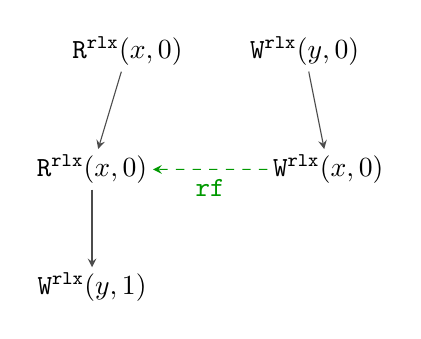
\begin{tikzpicture}[yscale=1.5,xscale=1.5]

    \node (xi) at (0.3,2) {$\rlab{\rlx}{x}{0}$};
    \node (yi) at (1.8,2) {$\wlab{\rlx}{y}{0}$};
    
    \node (rx) at (0,1) {$\rlab{\rlx}{x}{0}$};
    \node (wy) at (0,0) {$\wlab{\rlx}{y}{1}$};

    \node (wx) at (2,1) {$\wlab{\rlx}{x}{0}$};

    \draw[po] (xi)  edge  (rx);
    \draw[po] (yi)  edge  (wx);
    \draw[po] (rx)  edge  (wy);
    
    \draw[rf] (wx) edge node[below] {$\lRF$} (rx);
\end{tikzpicture}
\end{subfigure}
\begin{subfigure}{0.45\textwidth}
  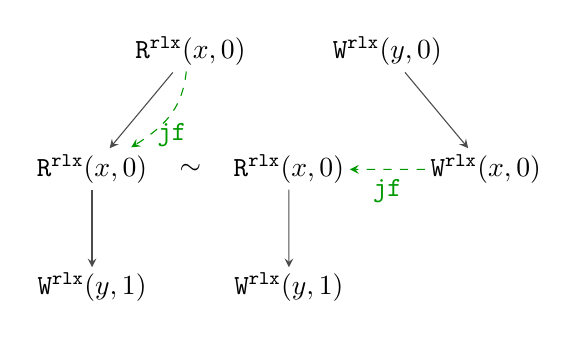
\begin{tikzpicture}[yscale=1.5,xscale=2.5]

    \node (xi) at (0.5,2) {$\rlab{\rlx}{x}{0}$};
    \node (yi) at (1.5,2) {$\wlab{\rlx}{y}{0}$};

    \node (rxa) at (0,1) {$\rlab{\rlx}{x}{0}$};
    \node (wya) at (0,0) {$\wlab{\rlx}{y}{1}$};

    \node (rxb) at (1,1) {$\rlab{\rlx}{x}{0}$};
    \node (wyb) at (1,0) {$\wlab{\rlx}{y}{1}$};

    \node (xcf) at (0.5,1) {$\sim$};

    \node (wx) at (2,1) {$\wlab{\rlx}{x}{0}$};

    \draw[po] (xi)  edge  (rxa);
    \draw[po] (yi)  edge  (wx);
    
    \draw[po] (rxa)  edge  (wya);
    \draw[po] (rxb)  edge  (wyb);

    \draw[rf] (xi) edge [bend left=20] node[below] {$\lJF$} (rxa);
    \draw[rf] (wx) edge node[below] {$\lJF$} (rxb);
\end{tikzpicture}
\end{subfigure}
\label{fig:rf-diff}
\end{figure}


\begin{figure}
\centering
\begin{subfigure}{1\textwidth}
\[\inarrIII{
  \incInst{\rlx}{\rlx}{r1}{x}{1}; ~\valueRead{0} \\
  \writeInst{\rlx}{y}{1};
}
{
  \readInst{\rlx}{r2}{z}; ~\valueRead{1} \\
  \writeInst{\rel}{x}{0};
}
{
  \incInst{\acq}{\rlx}{r3}{x}{1}; ~\valueRead{0} \\
  \writeInst{\rlx}{z}{1};
}\]
\end{subfigure}
\par\bigskip
\begin{subfigure}{1\textwidth}
  \begin{tikzpicture}[yscale=1.5,xscale=1.5]

    \node (ai) at (0.5,3) {$\rlab{\rlx}{x}{0}$};
    \node (bi) at (2.0,3) {$\wlab{\rlx}{y}{0}$};
    \node (ci) at (3.5,3) {$\wlab{\rlx}{y}{0}$};
    
    \node (aa) at (0,2) {$\rlab{\rlx}{x}{0}$};
    \node (ab) at (0,1) {$\wlab{\rlx}{x}{1}$};
    \node (ac) at (0,0) {$\wlab{\rlx}{y}{1}$};

    \node (ba) at (2,2) {$\rlab{\rlx}{z}{1}$};
    \node (bb) at (2,1) {$\wlab{\rel}{x}{0}$};

    \node (ca) at (4,2) {$\rlab{\acq}{x}{0}$};
    \node (cb) at (4,1) {$\wlab{\rlx}{x}{1}$};
    \node (cc) at (4,0) {$\wlab{\rlx}{z}{1}$};
    

    \draw[po] (ai)  edge  (aa);
    \draw[po] (bi)  edge  (ba);
    \draw[po] (ci)  edge  (ca);

    \draw[po]  (aa)  edge  (ab);
    \draw[po]  (ab)  edge  (ac);

    \draw[po] (ba)  edge  (bb);

    \draw[po] (ca)  edge  (cb);
    \draw[po] (cb)  edge  (cc);

    \draw[rmw] (aa)  edge[bend right=20] node[left] {$\lRMW$}  (ab);
    \draw[rmw] (ca)  edge[bend left=20] node[right] {$\lRMW$}  (cb);

    \draw[po] (cb)  edge  (cc);
    
    \draw[rf] (bb) edge node[below] {$\lRF$} (aa);
    \draw[rf] (ai) edge node[above] {$\lRF$} (ca);
    \draw[rf] (cc) edge node[below] {$\lRF$} (ba);
\end{tikzpicture}
\end{subfigure}
\par\bigskip
\begin{subfigure}{1\textwidth}
  \begin{tikzpicture}[yscale=1.5,xscale=1.5]

    \node (ai) at (2,3) {$\rlab{\rlx}{x}{0}$};
    \node (bi) at (4,3) {$\wlab{\rlx}{y}{0}$};
    \node (ci) at (6,3) {$\wlab{\rlx}{y}{0}$};
    
    \node (aa) at (0,2) {$\rlab{\rlx}{x}{0}$};
    \node (ab) at (0,1) {$\wlab{\rlx}{x}{1}$};
    \node (ac) at (0,0) {$\wlab{\rlx}{y}{1}$};

    \node (abcf) at (1,2) {$\sim$};

    \node (ba) at (2,2) {$\rlab{\rlx}{x}{0}$};
    \node (bb) at (2,1) {$\wlab{\rlx}{x}{1}$};
    \node (bc) at (2,0) {$\wlab{\rlx}{y}{1}$};

    \node (ca) at (4,2) {$\rlab{\rlx}{z}{1}$};
    \node (cb) at (4,1) {$\wlab{\rel}{x}{0}$};

    \node (da) at (6,2) {$\rlab{\acq}{x}{1}$};
    \node (db) at (6,1) {$\wlab{\rlx}{x}{2}$};
    \node (dc) at (6,0) {$\wlab{\rlx}{z}{1}$};

    \node (decf) at (7,2) {$\sim$};

    \node (ea) at (8,2) {$\rlab{\acq}{x}{0}$};
    \node (eb) at (8,1) {$\wlab{\rlx}{x}{1}$};
    \node (ec) at (8,0) {$\wlab{\rlx}{z}{1}$};
    

    \draw[po] (ai)  edge  (aa);
    \draw[po] (bi)  edge  (ca);
    \draw[po] (ci)  edge  (ea);

    \draw[po] (aa)  edge  (ab);
    \draw[po] (ab)  edge  (ac);

    \draw[po] (ba)  edge  (bb);
    \draw[po] (bb)  edge  (bc);

    \draw[po] (ca)  edge  (cb);

    \draw[po] (da)  edge  (db);
    \draw[po] (db)  edge  (dc);

    \draw[po] (ea)  edge  (eb);
    \draw[po] (eb)  edge  (ec);

    \draw[rmw] (aa)  edge[bend right=20] node[left] {$\lRMW$}  (ab);
    \draw[rmw] (ba)  edge[bend right=20] node[left] {$\lRMW$}  (bb);
    \draw[rmw] (da)  edge[bend left=20] node[right] {$\lRMW$}  (db);
    \draw[rmw] (ea)  edge[bend left=20] node[right] {$\lRMW$}  (eb);

    \draw[rf] (ai) edge[bend right=20] node[below] {$\lJF$} (aa);
    \draw[rf] (ab) edge node[below] {$\lJF$} (da);
    \draw[rf] (ai) edge node[above] {$\lJF$} (ea);
    \draw[rf] (cb) edge node[below] {$\lJF$} (ba);
    \draw[rf] (dc) edge node[below] {$\lJF$} (ca);
\end{tikzpicture}
\end{subfigure}
\label{fig:rf-rmw-diff}
\end{figure}


% \begin{proof}
  
% \end{proof}
  
\setmonofont[Mapping=tex-text]{CMU Typewriter Text}
\bibliographystyle{acm}
\bibliography{main.bib}

\end{document}
